\subsection{UML Class Diagram per tipi di dato}

\begin{center}
    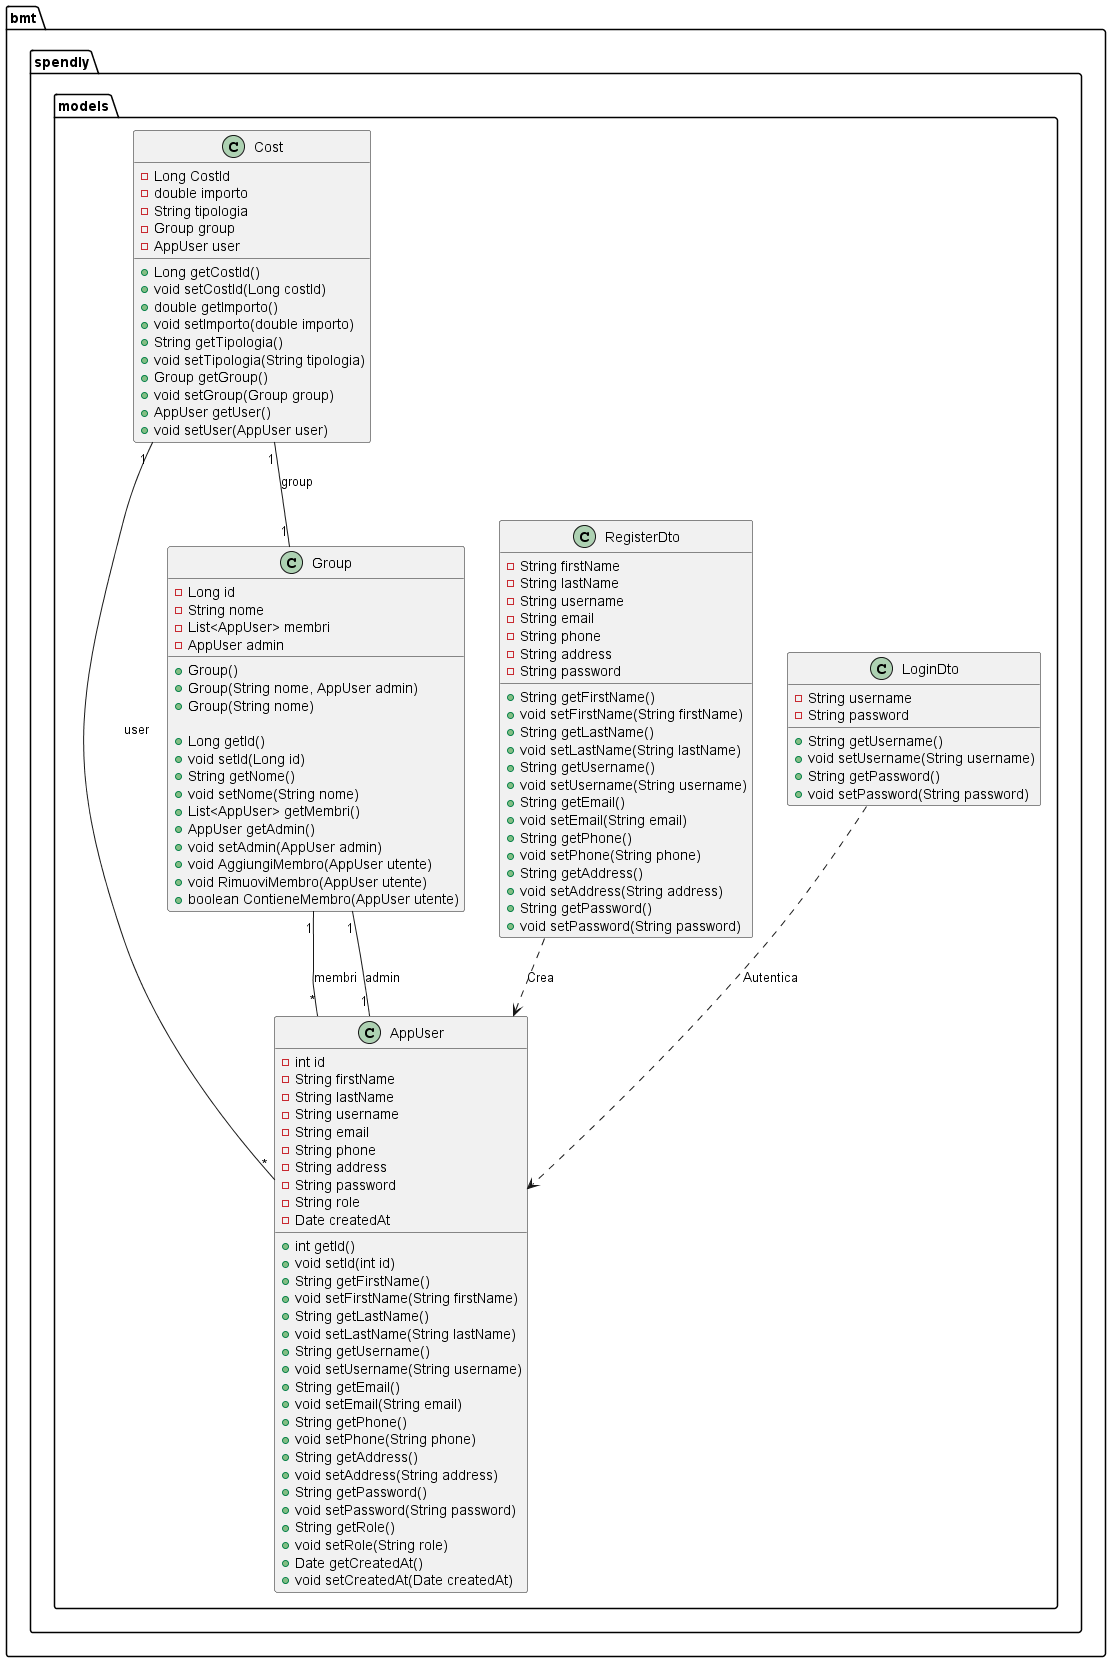
\includegraphics[scale=0.345]{images/ClassDiagram2.png}
\end{center}
\textbf{LoginDto $\rightarrow$ AppUser}: \begin{itemize} \item Rappresenta il processo di autenticazione nel sistema. \item La relazione mostra che la classe \texttt{LoginDto} contiene i dati necessari (username e password) per verificare l'identità di un utente già registrato (\texttt{AppUser}). \item In altre parole, \texttt{LoginDto} fornisce un mezzo per confermare che un utente (\texttt{AppUser}) ha accesso al sistema. \end{itemize}
\textbf{RegisterDto $\rightarrow$ AppUser}: \begin{itemize} \item Rappresenta il processo di registrazione di un nuovo utente. \item La relazione indica che la classe \texttt{RegisterDto} contiene i dati necessari (nome, cognome, email, password, ecc.) per creare un nuovo account utente (\texttt{AppUser}) all'interno del sistema. \item Questo significa che la classe \texttt{RegisterDto} viene utilizzata per tradurre i dati di registrazione in un'istanza valida della classe \texttt{AppUser}. \end{itemize}
\textbf{Group $\rightarrow$ AppUser (admin)}: \begin{itemize} \item Rappresenta il ruolo di amministratore per un gruppo. \item Ogni gruppo (\texttt{Group}) ha un amministratore specifico (\texttt{AppUser}) che è responsabile della gestione del gruppo. \item La relazione è uno-a-uno (1:1), il che significa che ogni gruppo ha un solo amministratore, ma un amministratore può gestire più gruppi. \item Questo legame indica che l'amministratore è una figura centrale per la gestione delle attività e dei membri del gruppo. \end{itemize}
\textbf{AppUser $\leftrightarrow$ Group (membri)}: \begin{itemize} \item Rappresenta i membri di un gruppo e la loro relazione con i gruppi. \item La relazione è molti-a-molti ($m:n$), il che significa che: \begin{itemize} \item Ogni utente (\texttt{AppUser}) può essere membro di più gruppi (\texttt{Group}). \item Allo stesso tempo, ogni gruppo può avere più utenti come membri. \end{itemize} \item Questo legame mostra che l'utente e il gruppo sono fortemente interconnessi, poiché i gruppi esistono per aggregare utenti, e gli utenti possono partecipare a più attività o comunità rappresentate dai gruppi. \end{itemize}
\textbf{Cost $\rightarrow$ Group}: \begin{itemize} \item Indica che un costo (\texttt{Cost}) può essere associato a un gruppo (\texttt{Group}). \item La relazione è molti-a-uno (1:n), il che significa che: \begin{itemize} \item Un costo appartiene a un singolo gruppo. \item Tuttavia, un gruppo può avere più costi associati. \end{itemize} \item Questa relazione consente di rappresentare costi condivisi o transazioni relative a un gruppo specifico. \end{itemize}
\textbf{Cost $\rightarrow$ AppUser}: \begin{itemize} \item Indica che un costo (\texttt{Cost}) è associato a un utente (\texttt{AppUser}). \item La relazione è molti-a-uno (1:n), il che significa che: \begin{itemize} \item Un costo è creato o sostenuto da un singolo utente. \item Tuttavia, un utente può avere più costi associati. \end{itemize} \item Questa relazione mostra che ogni costo ha un responsabile (l'utente) che lo ha sostenuto. \end{itemize}




